\documentclass[letterpaper,11pt]{article}

\usepackage{graphicx}% Include figure files
\usepackage{xcolor}

\textheight 22.cm
\textwidth 16.cm
\topmargin -1.7cm
\hoffset -1.5cm
\headsep 1.5cm
\parindent 1.2em
\baselineskip 16pt plus 2pt minus 2pt

\begin{document}

{\centering \bf \LARGE Proposal for Production of a Lattice QCD Data Visualization Code Base}

\section{Project Goal}
The goal for this project is to produce a code base that will provide all members of the
Lattice QCD (LQCD) group within FRIB the ability to perform basic LQCD data analyses and to visualize the analyses data
in a clear, efficient and robust way. As a byproduct of the data analysis,
it will also standardize our data formatting across our group members.

\section{Learning Outcomes}
The major motivation for this project is to provide our group with some skills in producing a code base in a group environment.
This project will also be useful for helping and sharing ideas and concepts of coding between group members.
Since this code base will be written in python (see Sec.~\ref{sec:imp}), utilizing some packages, we will gain the ability to
use python and the packages required for the project.

\section{Members and Time-frame}
The development will be performed by Jack Dragos, Jangho Kim, Giovanni Pederiva, Sam Liao, Matt Rizik and Mathias Vege (through zoom co-ordination).

The allocated time for development will be in our coding group meetings, typically held every Friday 10:30 am for approximately 1.5 hours.
\\ \hline \\
\vspace*{0.5cm}
\textcolor{red}{UPDATE meeting 28th September, 2018:} changed meetings to be allocated for updating on the project and to plan for the proceeding week of work.
This means that the coding will be done between meetings.
\\ \hline \\
\vspace*{0.5cm}
A time frame review will be performed in 3 months time (7th December) to review progress, discuss any alterations in design and to determine
if the project will be continued.

This proposal was produced in the first meeting, the following meetings are planned to undertake the following:

\begin{itemize}
  \item Meeting to understand bokeh and pyvis python packages for plotting (see Sec.~\ref{sec:pack}).
  \item Meeting to discuss data structure and IO.
  \item Meeting to decide on delegating sections of code to group members.
\end{itemize}

\section{Implementation \label{sec:imp}}

\subsection{Code Structure/Graph}
Referring to fig.~\ref{code_sch}, data is main class type for reading in data and all our types of data
(e.g. two-point correlators, flowed opeartors etc...) is inherited from Data.
A "pyvis settings" class will then take in a Data object instance which will control the GUI interface for data visualization.
IO will be done in pyvis, which will link to IO within the Data class.
\begin{figure}
  \centering
  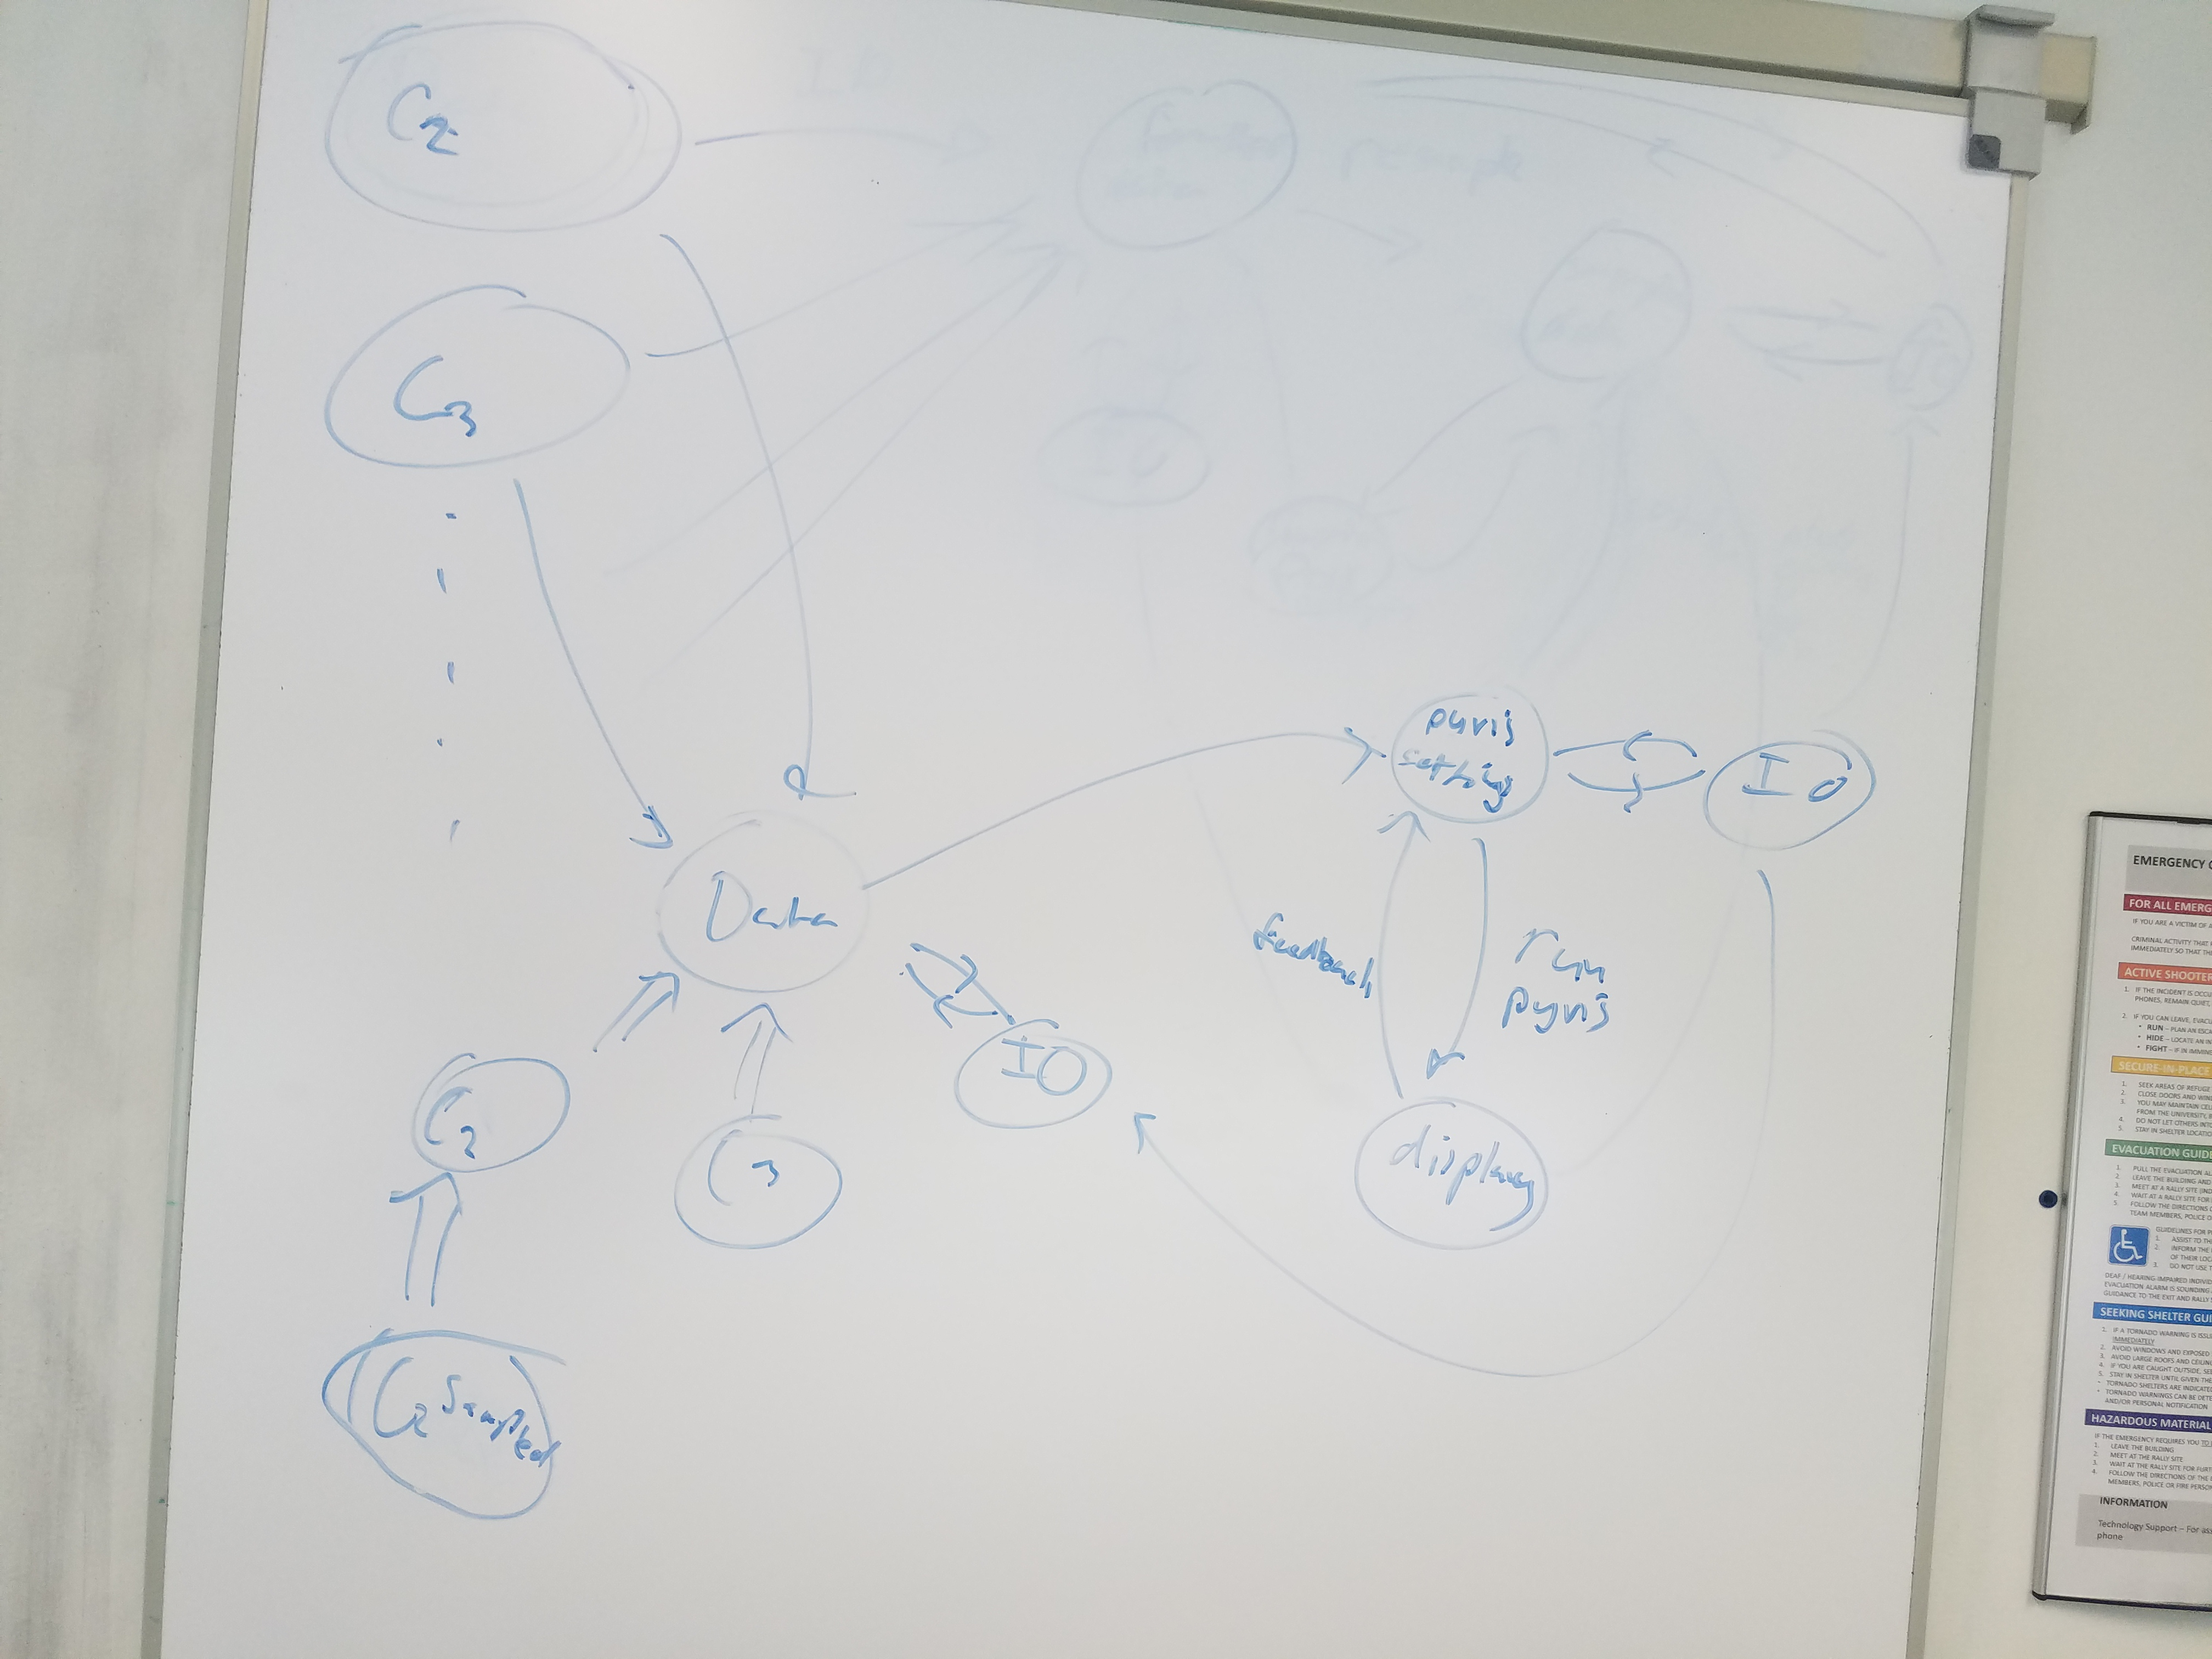
\includegraphics[trim={20cm 0cm 20cm 0cm},clip,width=\linewidth]{/home/jackdra/LQCD/Scripts/group_meeting/Data_Vis_Proj/Plan/Code_Schematic}
  \caption{\label{code_sch}Code schematic for code base. }
\end{figure}
\subsection{Data IO Standardization}


The Data class and each child subclass will have its own IO function. Along with this, the "pyvis settings" class will have its own
IO class, which will link to the IO of the Data objects used in the figures.

All storage of Data objects will be in hdf5 for efficiency and usability. The data stored for pyvis will (most likely) be in JSON formatting
for human readability.
\\ \hline \\
\vspace*{0.5cm}
\textcolor{red}{UPDATE meeting 28th September, 2018:} xarray data type has been addopted, this means netCDF (built on top of hdf5) is addpoted for binary data storage.
\\ \hline \\
\vspace*{0.5cm}


\subsection{Language and Packages \label{sec:pack}}
This project will be written in Python version 3.6, with no planned backwards compatibility with version 2.7.

The project will use the following packages.
\begin{itemize}
  \item numpy:    Basic array and number manipulation
  \item pandas:   Primary method for storing data in tabulated form. Provides inbuilt IO functions as well.
  \item bokeh:    Back end for plotting, used in substitute for matplotlib to provide web based plot display and greater formatting and functionality.
  \item holoviews     Package built on bokeh used for greater functionality for plotting.
\end{itemize}

\subsection{Debugging, Testing and Test Sets}
Since all types of data computed from CHROMA will be child classes of a master Data class, sample data
for this class will be produced to be used for debugging Data and "pyvis settings" classes.
We will need some raw CHROMA data to test IO for all the child classes of Data.

\section{Roles/Delegation}
This is to be decided in (the planned) 3 weeks time, after we have done some preliminary testing on pyvis, bokeh and discussed standardized
IO data formatting.
\\ \hline \\
\vspace*{0.5cm}
\textcolor{red}{UPDATE meeting 28th September, 2018:}
\begin{itemize}
  \item Matt and Jack are delegated to the "data" part of the code.
  \item Giovanni and Sam will be working on the "visualisation" part of the code.
  \item Jangho has agreed to provide support and possible testing/debugging with the project.
\end{itemize}
\\ \hline \\
\vspace*{0.5cm}


\end{document}
